\documentclass{beamer}
\mode<presentation> 
{
	\usetheme[alternativetitlepage]{Torino}
	\usecolortheme{chameleon}
	\setbeamercovered{transparent}	
}
\definecolor{olive}{RGB}{51, 149, 48}
\definecolor{red}{RGB}{195, 2, 36}

\usepackage{ucs}
\usepackage[utf8x]{inputenc}
\usepackage[czech]{babel}
\usepackage{palatino}
\usepackage{graphicx}
\usepackage{epstopdf}
\usepackage{color}
\usepackage[export]{adjustbox}
\usepackage{multicol}
\usepackage{hyperref}
\usepackage[labelfont={color=olive,scriptsize}]{caption}
\usepackage{subcaption}




\title{\large{\textbf{Detekce hran s využitím dynamického programování}}}
\subtitle{\small{představení projektu}}
\author{Pavel Macenauer \\ \tiny{pavel.macenauer@fotoaparat.cz} \\ \normalsize{Jan Bureš} \\ \tiny{xbures19@stud.fit.vutbr.cz}}
\date{\tiny{\today}}
\institute[FIT VUTBR]
{
	\inst{}
	Fakulta Informačních Technologií \\
	Vysoké Učení Technické v Brně
}

\begin{document}

	\begin{frame}[t,plain]
	\titlepage

	\vspace{-7mm}
	\center{ 
\includegraphics[height=7mm]{logo.eps} }
	\end{frame}

%% ------------- princip -------------

	\begin{frame}[t,fragile]
		\frametitle{Princip detekce hran pomocí dynamického programování}	
	\centering{		
	\begin{figure}[h!]
	

	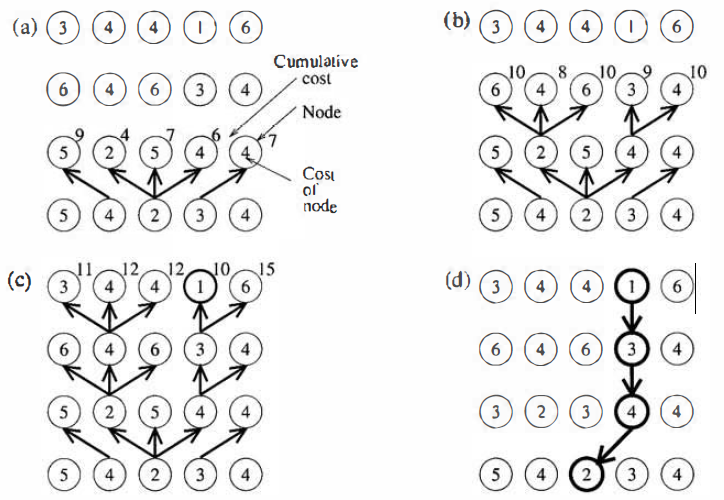
\includegraphics[height=47mm]{theory.png}
	\caption{\scriptsize{\textcolor{red}{(a)}-\textcolor{red}{(c)} Pro každý uzel se spočítá ohodnocení pomocí vhodné funkce a postupně se počítají optimální cesty z předchozích uzlů \textcolor{red}{(d)} nejlepší cesta se určí backtracingem. Uzly můžou reprezentovat pixely a ohodnocení např. inverzi jasu.}}
		\end{figure}					  		
		}
	\end{frame}
	
	%% ------------- cil a rozdeleni projektu -------------

	\begin{frame}[t,fragile]
		\frametitle{Cíle projektu}	

		\begin{itemize}
			\item Prozkoumat do detailu jak funguje detekce hran pomocí dynamického programování
			\item Prozkoumat vyhodnocovací funkce
			\item Implementovat detektor hran v C++ a OpenCV na základě předchozí analýzy
			\item Vyhledat testovací obrázky a otestovat funkčnost programu
			\item V dokumentaci analyzovat výsledky
		\end{itemize}
	\end{frame}
	
	
	\begin{frame}[t,fragile]
		\frametitle{Rozdělení projektu}	

		\begin{itemize}
			\item \textcolor{red}{Pavel Macenauer}
			\begin{itemize}
				\item Založení vývojového prostředí (Git, Skype, ...)
				\item Průzkum detekce hran pomocí dynamického programování, ohodnocovacích funkcí a vyhledávání materiálu
				\item Implementace základní kostry programu, výpočetních struktur a následné vykonnostní optimalizace
				\item Dokumentace
			\end{itemize}
			\item \textcolor{red}{Jan Bureš}
			\begin{itemize}							
				\item Průzkum detekce hran pomocí dynamického programování, ohodnocovacích funkcí a vyhledávání materiálu
				\item Implementace vyhodnocování uzlů, průchodu strukturou a backtrackingu
			\end{itemize}
		\end{itemize}
		
	\end{frame}
	
\end{document} 
